% ----------------------------------------------------------
\chapter{Algoritmos e estruturas de dados para consulta de pontos no plano}\label{cap:desenvolvimento}
% ----------------------------------------------------------
Nesta seção veremos formas de construir estruturas de dados para um conjunto de pontos no plano. 
Consideramos que os pontos são fixos. Para cada estrutura construída, veremos também como utilizá-la para
consultar pontos dentro de uma janela.

% ----------------------------------------------------------
\section{Árvore KD}
% ----------------------------------------------------------

Uma árvore KD é uma árvore binária onde cada folha é um ponto \textit{k-dimensional}.
Cada nó não-folha guarda um valor $v$ em uma dimensão $d$.
Pontos cujo os valores na dimensão $d$ são iguais ou menores a $v$ estão na subárvore à esquerda de $v$,
e respectivamente, pontos maiores que $v$ com valores na dimensão $v$ estão para o lado direito.
Cada nível da árvore é associado a uma das \textit{k dimensões}. Então, a citar um exemplo no plano, se dado nó
 divide o eixo
$x$, a subárvore à esquerda contém os pontos com o eixo $x$ menor que o valor $v$. Similarmente,
 ã direita contém os pontos com o eixo $x$ maior que o valor $v$. 

\subsection{Árvore 2D}
Uma árvore 2D é a versão com duas dimensões para árvores KD. A sua construção considera um conjunto 
de pontos no plano dado ($P$) e pode ser feita da seguinte forma.

Na construção de uma árvore para 2 dimensões, cada ponto tem uma forma $p : (p_x, p_y)$ .
Escolhemos um eixo para iniciar a construção da árvore. Ao iniciar a construção da arvore,
realizamos uma $x$-ordenação e uma $y$-ordenação nos pontos de $P$ (no caso $n$ dimensional, faremos
$n$-ordenações). Chamaremos o conjunto de pontos ordenados pelo eixo $x$ de $P_{ordenado(x)}$, e ordenados por $y$ de 
$P_{ordenado(y)}$.

O \cite{cg08} valor da mediana dos pontos ordenados pelo eixo será o valor de corte do conjunto $P$,
e serão criados dois subconjuntos.
Chama-se recursivamente a construção das subárvores à esquerda e à direita de $v$ alternando o eixo 
e passando os subconjuntos. Considere o seguinte conjunto de pontos.

\begin{center}
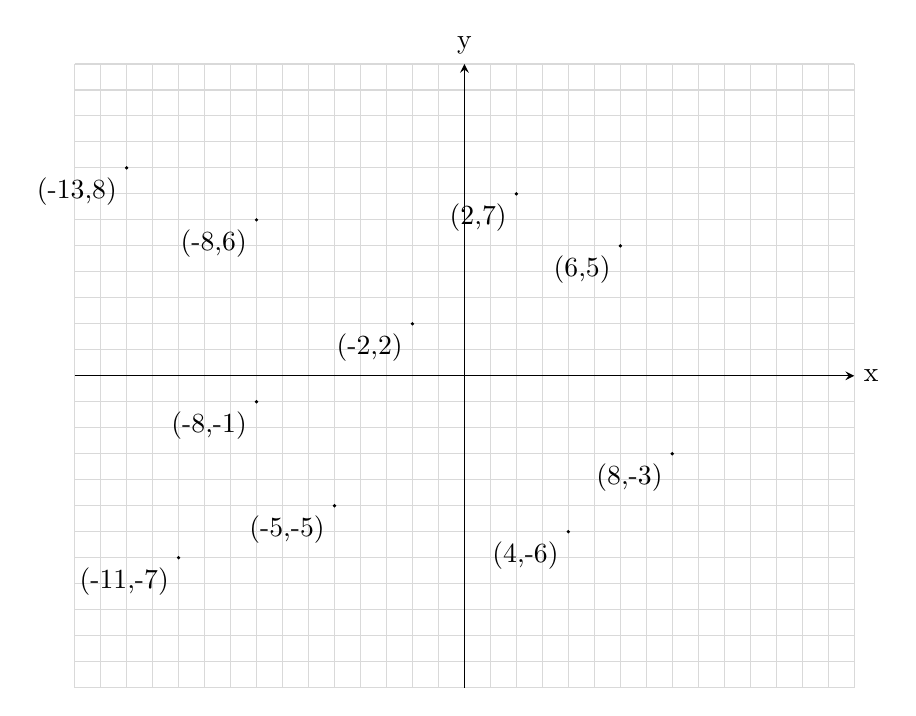
\begin{tikzpicture}[scale=0.33]
  \draw[gray!30] (-15,-12) grid[xstep=1, ystep=1]  (15,12);
  \draw[-stealth] (-15,0)--(15,0) node[right]{x}; % x axis
  \draw[-stealth] (0,-12)--(0,12) node[above]{y}; % y axis


  \fill (-13,8)  circle[radius=2pt] node[anchor=north east]{(-13,8)};
  \fill (-8,6)  circle[radius=2pt] node[anchor=north east]{(-8,6)};
  \fill (-2,2)  circle[radius=2pt] node[anchor=north east]{(-2,2)};
  \fill (-8,-1)  circle[radius=2pt] node[anchor=north east]{(-8,-1)};
  \fill (-11, -7)  circle[radius=2pt] node[anchor=north east]{(-11,-7)};
  \fill (-5,-5)  circle[radius=2pt] node[anchor=north east]{(-5,-5)};
  \fill (2,7)  circle[radius=2pt] node[anchor=north east]{(2,7)};
  \fill (6,5)  circle[radius=2pt] node[anchor=north east]{(6,5)};
  \fill (8,-3)  circle[radius=2pt] node[anchor=north east]{(8,-3)};
  \fill (4,-6)  circle[radius=2pt] node[anchor=north east]{(4,-6)};
\end{tikzpicture}
\qquad
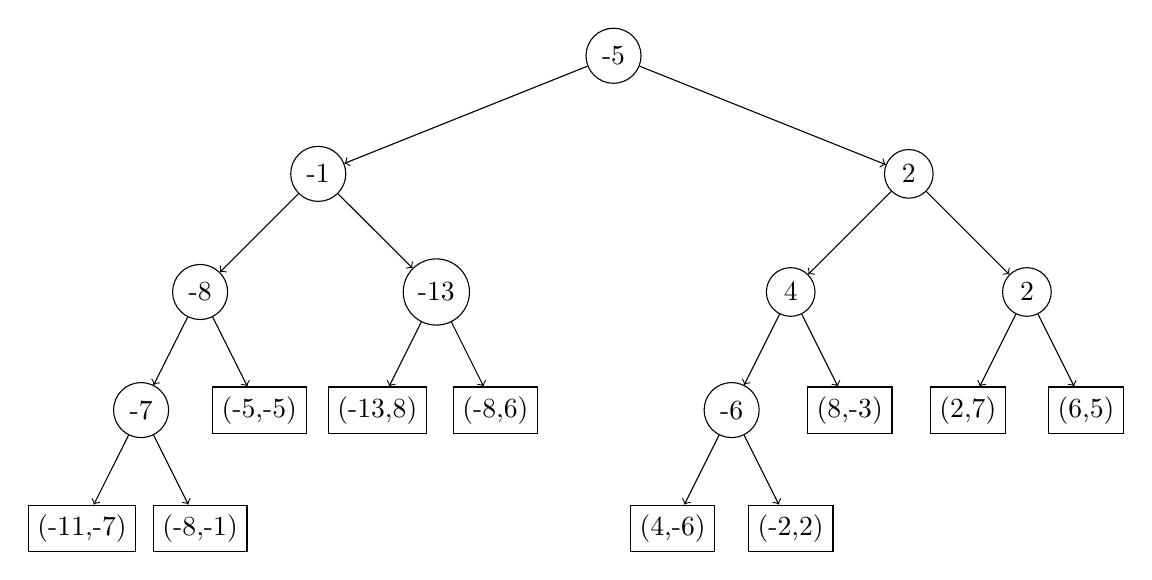
\begin{tikzpicture}[nodes={draw, circle}, ->]
    % Tree structure
 \node{-5}
    child { node {-1} 
        child { node {-8}
            child{ node{-7}
                child{ node[rectangle]{(-11,-7)}}
                child{ node[rectangle]{(-8,-1)}}
            }
            child { node[rectangle]{(-5,-5)}}
        }
        child [missing]
        child { node {-13}
            child { node[rectangle]{(-13,8)}}
            child { node[rectangle]{(-8,6)}}
        }
    }
    child [missing]
    child [missing]
    child [missing]
    child [missing]
    child { node {2} 
        child { node {4}
            child{node{-6}
                child {node[rectangle]{(4,-6)}  }
                child {node[rectangle]{(-2,2)}  }
            }
            child{node[rectangle]{(8,-3)}}
        }
        child [missing]
        child { node{2}
            child{node[rectangle]{(2,7)}}
            child{node[rectangle]{(6,5)}}
        }
    };
\end{tikzpicture}

\end{center}

Inicialmente escolhemos o eixo-$x$. Acompanharemos a troca de eixos segundo a profundidade da árvore.
Caso a profundidade seja $par$, consideramos o eixo $x$, do contrário eixo $y$.
Como temos $P_{ordenado(x)}$, sabemos que o ponto médio representará o valor $x_{mediana}$.

Criamos dois subconjuntos $P_1$ e $P_2$ tal que:

    $P_1 = \{p \in P : p_x \leq x_{mediana}\}$ e $P_2 = \{p \in P : p_x > x_{mediana}\}$.

Agora, recursivamente, repete-se para os dois novos conjuntos criados e considerar $y$ até restar 
somente um ponto. Este, por sua vez, será um nó folha da árvore e tratado na base da recursão. 
O pseudocódigo para a construção de uma árvore 2D é dado em seguida.

\begin{algorithm}
    \caption{O algorítimo \Call{ConstroiArvore2D}{$P$, $profundidade=0$}, recebe um conjunto de 
    pontos $P$ no plano e uma profundidade da árvore.
    O algoritmo retorna a raiz de uma árvore 2D}
    \begin{algorithmic}[1]
        \Function{ConstroiArvore2D}{$P$, $profundidade$}
            \If{P contem apenas um ponto}
            \Return $nó \leftarrow ponto$
        \Else
            \If{$profundidade$ é par}
            \State
                Divide P em dois subconjuntos com um linha vertical $l$ pela mediana da $x$-coordenada
                dos pontos em P. Seja $P_1$ o conjunto dos pontos à esquerda de $l$ e seja
                $P_2$ o conjunto de pontos à direita de $l$.
            \Else
            \State
                Divide P em dois subconjuntos com um linha horizontal $l$ pela mediana da $y$-coordenada
                dos pontos em P. Seja $P_1$ o conjunto dos pontos abaixo de $l$ e seja
                $P_2$ o conjunto de pontos acima de $l$.
            \EndIf
        \EndIf
        \State Cria os nós $v_{esquerda}$ e $v_{direita}$
        \State $v_{esquerda} \leftarrow $ \Call{ConstroiArvore2D}{$P_1, profundidade+1$}
        \State $v_{direita} \leftarrow $ \Call{ConstroiArvore2D}{$P_2, profundidade+1$}
        \State Cria um nó $v$, associamos o valor $l$ e associamos os filhos $v_{esquerda}$ e $v_{direita}$ 

        \Return $v$
        \EndFunction
    \end{algorithmic}
\end{algorithm}

\clearpage


\subsection{Consulta}
Uma consulta 2-dimensional em $P$ é uma busca de quais pontos de $P$ da busca estão
entre um retângulo de consulta \([x,x']  \times  [y,y']\). 
Um ponto $p:= (p_x, p_y)$ está dentro de um retângulo de busca se e somente se:

\[
p_x \in [x, x'] \textrm{ e } p_y \in [y, y']
\]

Podemos dizer que uma consulta 2-dimensional é composta de duas sub-consultas 1-dimensional: uma no
eixo \(x\) de um dos pontos e uma consulta no eixo \(y\).

\begin{figure}[htb]
    \caption{\label{fig:Fig_2}Busca em alcance \textit{dimensional} - 2D}
    \begin{center}
        \includegraphics{images/search_range.png}
    \end{center}
\end{figure}


Denotaremos esta área de um nó \(v\) como \(região(v)\). A região da raiz é (no caso de uma árvore 2D) 
o plano inteiro.
Portanto, o algoritmo buscará pela subárvore com raiz \(v\) somente se o retângulo de busca intersectar
a \(região(v)\).


Como cada nó $v$ tem um intervalo de pontos em suas folhas, denotaremos a área do nó $v$ sendo o intervalo:

Seja $P_v$ o conjunto de pontos em $v$ (os nós folha alcançáveis de $v$). Seja $p \in P_v$:

\begin{center}
 \mbox{
    área_v =  \begin{cases} p_{x min} \leq x \leq p_{x max} \\ p_{y min} \leq y \leq p_{y max} \end{cases} 
}
\end{center}


A área do $nó_4$ é igual:
\begin{center}
 \mbox{
    área_4 =  \begin{cases} -2 \leq x \leq 8 \\ -6 \leq y \leq 2 \end{cases} 
}
\end{center}

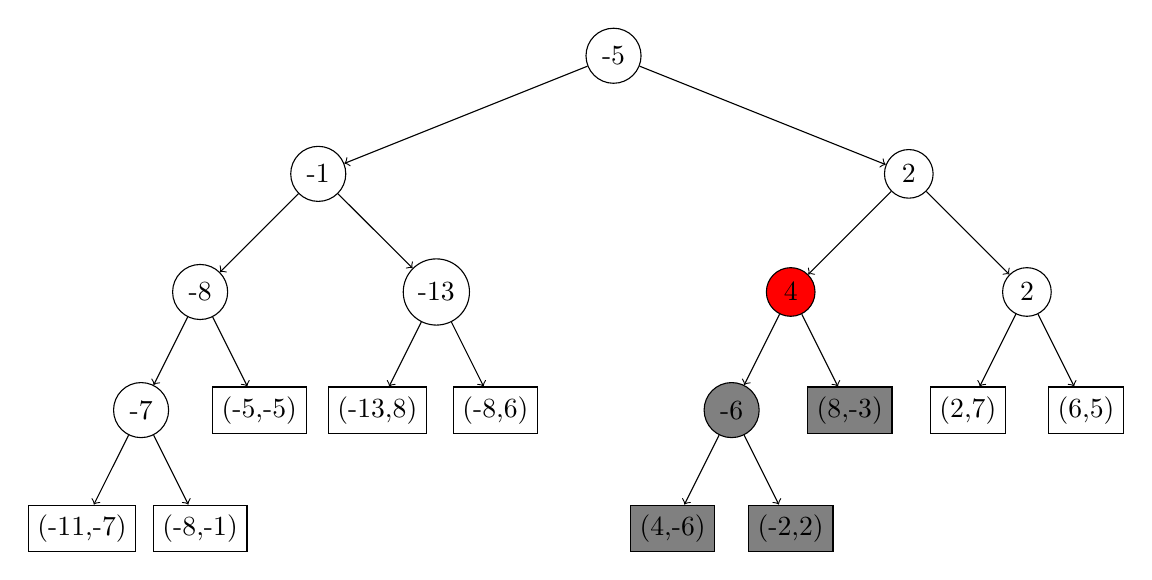
\begin{tikzpicture}[nodes={draw, circle}, ->]
 
    % Tree structure
 \node{-5}
    child { node {-1} 
        child { node {-8}
            child{ node{-7}
                child{ node[rectangle]{(-11,-7)}}
                child{ node[rectangle]{(-8,-1)}}
            }
            child { node[rectangle]{(-5,-5)}}
        }
        child [missing]
        child { node {-13}
            child { node[rectangle]{(-13,8)}}
            child { node[rectangle]{(-8,6)}}
        }
    }
    child [missing]
    child [missing]
    child [missing]
    child [missing]
    child { node {2} 
        child { node[fill=red]{4}
            child{node[fill=gray]{-6}
                child {node[rectangle, fill=gray]{(4,-6)}  }
                child {node[rectangle ,fill=gray]{(-2,2)}  }
            }
            child{node[rectangle, fill=gray]{(8,-3)}}
        }
        child [missing]
        child { node{2}
            child{node[rectangle]{(2,7)}}
            child{node[rectangle]{(6,5)}}
        }
    };
\end{tikzpicture}

O algoritmo de busca funciona descendo a árvore, mas visitando somente os nós que a
\(região(v)\) intersecta o retângulo da consulta. Quando uma \(região(v)\) está contida na
janela de busca devolvemos todos os pontos na subárvore.
Quando chegarmos nos nós folha temos de checar se o nodo esta dentro da consulta, se estiver,
devolvê-lo.



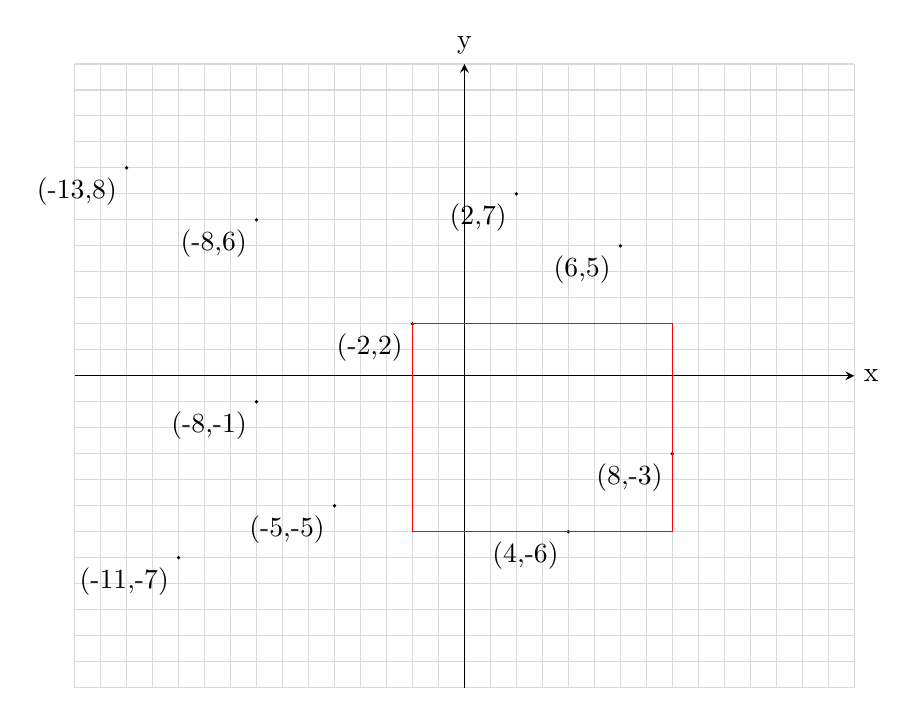
\begin{tikzpicture}[scale=0.33]
  \draw[gray!30] (-15,-12) grid[xstep=1, ystep=1]  (15,12);
  \draw[-stealth] (-15,0)--(15,0) node[right]{x}; % x axis
  \draw[-stealth] (0,-12)--(0,12) node[above]{y}; % y axis


  \fill (-13,8)  circle[radius=2pt] node[anchor=north east]{(-13,8)};
  \fill (-8,6)  circle[radius=2pt] node[anchor=north east]{(-8,6)};
  \fill (-2,2)  circle[radius=2pt] node[anchor=north east]{(-2,2)};
  \fill (-8,-1)  circle[radius=2pt] node[anchor=north east]{(-8,-1)};
  \fill (-11, -7)  circle[radius=2pt] node[anchor=north east]{(-11,-7)};
  \fill (-5,-5)  circle[radius=2pt] node[anchor=north east]{(-5,-5)};
  \fill (2,7)  circle[radius=2pt] node[anchor=north east]{(2,7)};
  \fill (6,5)  circle[radius=2pt] node[anchor=north east]{(6,5)};
  \fill (8,-3)  circle[radius=2pt] node[anchor=north east]{(8,-3)};
  \fill (4,-6)  circle[radius=2pt] node[anchor=north east]{(4,-6)};
  \draw[draw=red] (-2,-6) rectangle (8,2);

\end{tikzpicture}

Segue o algoritmo que recebe como parâmetros a raiz da arvore2D e o retângulo de consulta \(R\).
Usamos uma chamada \(RetornaSubárvore(v)\) que atravessa a árvore do nó \(v\) e retorna
todos os pontos nas suas folhas. Segue como notação \(filho_{esquerda}(v)\) sendo o filho da esquerda e
\(filho_{direita}(v)\) o filho da direita do nó \(v\).


\begin{algorithm}[H]
    \caption{A função \Call{BuscaEmArvore2D}{$v$, $consulta$} recebe como parâmetro um nó e uma 
    consulta.
     E retorna todos os pontos dentro da consulta.}
    \begin{algorithmic}[1]
    \Function{BuscaEmArvore}{$v$, $consulta$}
        \If{v é folha}
        \Return  $v$ se estiver dentro da $consulta$
        \Else
            \If{$região(filho_{esquerda}(v))$ está contido na $consulta$}
            \State \Return $Subárvore( filho_{esquerda}(v) )$
            \Else
                \If{$região(filho_{esquerda}(v))$ intersecta $consulta$}
                \State \Call{BuscaEmArvore2D}{$filho_{esquerda}(v)$, $consulta$}
                \EndIf
            \EndIf
            \If{$região(filho_{direita}(v))$ está contido na $consulta$}
            \State \Return $Subárvore(filho_{direita}(v))$
            \Else
                \If{$região(filho_{direita}(v))$ intersecta $busca$}
                \State \Call{BuscaEmArvore2D}{$filho_{direita}(v)$, $consulta$}
                \EndIf
            \EndIf
        \EndIf
    \EndFunction
    \end{algorithmic}
\end{algorithm}

\subsection{Construindo uma Árvore 2D}
Sejam os pontos da Figura 3, os pontos, segue a construção da árvore.
Fazemos uma $x$-ordenação pelos pontos e obtemos a seguinte ordenação:
\[
    (-13,8), (-11,-7), (-8,6), (-8,-1), (-5,5), (-2, 2), (2,7), (4,-6),(6,5),(8,-3)
\]
Calculamos que o valor da mediana será $(-5,5)$ e seguimos a seguinte convenção:
Seja $n$ o comprimento da lista de pontos, a subárvore à esquerda terá os pontos $0 < x \leq 
\frac{n-1}{2}$ e a subárvore a direita terão, respectivamente, os pontos $ \frac{x-1}{2} > x \geq n -1$

Criamos um nó raiz com o valor $-5$, dividimos o conjunto de pontos em dois subconjuntos: $P_1$ 
com os pontos com $x \leq -5$ e $P_2$ com os pontos $x > -5$.
Criamos dois nodos: $v_{esquerda}$ $v_{direita}$, e associamos os conjuntos $P_1$ e $P_2$ na chamadas
recursivas: 

A área do nó raiz é calculada como: 
$ -13 \leq x \leq 8 $ e $ -7 \leq y \leq 8$. 

\begin{tikzpicture}[x=0.25cm,y=0.25cm]
%   \draw[gray!30] (-15,-12) grid[xstep=1, ystep=1]  (15,12);
  \draw[-stealth] (-15,0)--(15,0) node[right]{x}; % x axis
  \draw[-stealth] (0,-12)--(0,12) node[above]{y}; % y axis

\draw[red] (-5,12)--(-5,-12); % y axis

  \fill (-13,8)  circle[radius=2pt] ;
  \fill (-8,6)  circle[radius=2pt] ;
  \fill (-2,2)  circle[radius=2pt] ;
  \fill (-8,-1)  circle[radius=2pt];
  \fill (-11, -7)  circle[radius=2pt];
  \fill (-5,-5)  circle[radius=2pt] node[anchor=north east]{(-5)};
  \fill (2,7)  circle[radius=2pt] ;
  \fill (6,5)  circle[radius=2pt] ;
  \fill (8,-3)  circle[radius=2pt];
  \fill (4,-6)  circle[radius=2pt];
\end{tikzpicture}

E agora repete-se o procedimento para os subconjuntos $P_1$ e $P_2$.
Para os pontos de $P_1$, como a profundidade é ímpar, agora faz-se uma $y$-ordenação e calcula-se a mediana:
\[
    (-11,7), (-5,-5), (-8,-1), (-8,6), (-13,8)
\]

Temos que a mediana é $(-8,-1)$, portanto criamos um nó com o valor $-1$. Dividimos o conjunto de 
pontos em $P_1 \leftarrow (-11,7), (-5,-5), (-8,-1) $ e $P_2 \leftarrow (-8,6), (-13,8)$.
Calculamos a área do nó sabendo qual o valor de corte do nó pai.
Sabemos que o eixo foi cortado em $-5$ em $x$.
Calcularemos a área do $nó_{-1}$
\[
    -11 \leq x < -5 \textmd{ e } -5 \leq y < 8
\] 

\begin{tikzpicture}[x=0.25cm,y=0.25cm]
%   \draw[gray!30] (-15,-12) grid[xstep=1, ystep=1]  (15,12);
  \draw[-stealth] (-15,0)--(15,0) node[right]{x}; % x axis
  \draw[-stealth] (0,-12)--(0,12) node[above]{y}; % y axis
  \draw[red] (-5,12)--(-5,-12); % y axis
  \draw[green] (-15,-1)--(-5,-1); % y axis
  \fill (-13,8)  circle[radius=2pt] ;
  \fill (-8,6)  circle[radius=2pt] ;
  \fill (-2,2)  circle[radius=2pt] ;
  \fill (-8,-1)  circle[radius=2pt] node[anchor=north east]{(-1)};
  \fill (-11, -7)  circle[radius=2pt];
  \fill (-5,-5)  circle[radius=2pt] ;
  \fill (2,7)  circle[radius=2pt] ;
  \fill (6,5)  circle[radius=2pt] ;
  \fill (8,-3)  circle[radius=2pt];
  \fill (4,-6)  circle[radius=2pt];
\end{tikzpicture}

Repete-se recursivamente o procedimento até o conjunto $P$ na chamada \Call{ConstroiArvore2D}{$P$, $prof$}
contiver somente um ponto. Cria-se então um nó folha, contendo como valor o ponto $p$.


Para realizarmos uma busca na árvore construída, com uma consulta $ -3 \leq x \leq 9 $ e $-7 \leq y < 3$.
Iniciamos no nó $-5$. Como o nó não é folha, checamos se a área do filho à esquerda esta dentro da consulta.
O $nó_{-1}$ tem área $ -13 \leq x \leq -5 $ e  $ -7 \leq y \leq 8$, logo a área não está contida 
na consulta.

A área dos nós $nó_2$ e $nó_{-1}$ intersectam a consulta, então procedemos chamando
\Call{BuscaEmArvore}{$nó_{-1}$, consulta} e \Call{BuscaEmArvore}{$nó_{2}$, consulta}.

O $nó_{2}$, o $filho_{esquerda}$ é o $nó_4$, que está contido na área da consulta e portanto todos
os pontos folha são retornados.


A Figura 5 corresponde a uma figura gerada por nossas implementações da árvore 2D. Como esperado, os
pontos dentro de uma janela foram retornados.
\begin{figure}[H]
    \caption{\label{fig:Fig_5} — Resultados de busca com Arvore2D}
    \begin{center}
        \includegraphics{images/points.pdf}
    \end{center}
\end{figure}
\clearpage



% ----------------------------------------------------------
\section{Arvore de Alcance}
% ----------------------------------------------------------

Uma árvore de alcance é uma árvore binária para buscas $n$-dimensional que possui demais árvores aninhadas
nas $n$-dimensões.
Cada nó não-folha é um valor $v$ em uma dimensão $d$, associado ã uma segunda arvore indexada pelo o 
eixo $d_2$.

Sendo a consulta $n$-dimensional uma junção de $n$-consultas unidimensional.

Uma árvore de alcance $2-dimensional$ é uma árvore indexada inicialmente pelo eixo $x$, e para cada
nó não-folha, associa-se uma árvore binária indexada pelo eixo $y$.

A consulta consiste em encontrar o nó $v$ menor ancestral comum dos pontos da consulta, e quando encontrar este
ponto, para os $filhos_{esquerda}$ deste $v$, retorna todos os $pontos_{direita}$. E para os $filhos_{direita}$
de $v$ retorna todos os pontos à esquerda.

\begin{figure}[htb]
    \caption{\label{fig:Fig_6} — Arvore de Alcance 2D}
    \begin{center}
        \includegraphics{images/range_tree.pdf}
    \end{center}
\end{figure}


% ----------------------------------------------------------